\definecolor{codebg}{RGB}{248,249,250}
\definecolor{codeframe}{RGB}{220,223,228}
\definecolor{codekw}{RGB}{25,85,145}
\definecolor{codecm}{RGB}{90,125,90}
\definecolor{codestr}{RGB}{136,44,136}
% Java代码风格
\lstdefinestyle{cleanjava}{
  language=Java,
  basicstyle=\ttfamily\small,
  keywordstyle=\bfseries\color{codekw},
  commentstyle=\itshape\color{codecm},
  stringstyle=\color{codestr},
  backgroundcolor=\color{codebg},
  frame=single,
  rulecolor=\color{codeframe},
  framesep=6pt,
  numbers=left,
  numberstyle=\scriptsize\color{gray},
  numbersep=8pt,
  breaklines=true,
  breakatwhitespace=false,
  showstringspaces=false,
  keepspaces=true,
  tabsize=4,
  columns=fullflexible
}


\chapter{实验目的}
本实验旨在通过开发一个基于命令行的个人所得税计算程序，系统性锻炼面向对象程序设计能力，深入理解封装、信息隐藏、数据抽象、异常处理等核心机制，并养成良好的编码规范和工程化习惯。具体目标如下：
\begin{itemize}
	\item \textbf{掌握面向对象设计方法：} 通过将个税计算问题抽象为多个类，体会高内聚、低耦合、分层设计思想，提升系统建模与分工协作能力。
	\item \textbf{强化编译原理知识联系：} 在项目开发过程中，结合词法、语法、语义分析等编译原理知识，理解程序结构、数据流与异常处理的本质联系。
	\item \textbf{规范编程与文档习惯：} 严格遵循 Java 编码规范，注重代码风格、注释完整性和文档化，提升代码可维护性和团队协作能力。
	\item \textbf{提升实际编程能力：} 通过需求分析、系统设计、编码实现、单元测试和异常处理等完整流程，提升独立开发和问题解决能力。
	\item \textbf{注重健壮性与用户体验：} 通过输入校验、异常捕获和友好提示，保证程序健壮性和良好用户体验。
	\item \textbf{为后续扩展打基础：} 通过合理的结构设计和模块划分，为后续支持多种税制、图形界面等功能扩展提供良好基础。
\end{itemize}
通过本实验，不仅能够加深对编译原理相关知识的理解，还能全面提升面向对象设计、Java 编程、规范文档和实际工程能力。

\chapter{实验环境}
\section{编程语言}
Java（JDK 1.5及以上）
\section{开发工具}
支持 Eclipse、VS Code、命令行等多种开发环境，最终程序可直接用 JDK 编译运行。
\section{编码规范}
严格遵循 Sun/Oracle Java 编码规范，采用驼峰命名法，类、方法、变量命名规范，注释完整，结构清晰。
\subsection{标识符命名}
本项目严格遵循 Sun/Oracle Java 编码规范，采用驼峰命名法（CamelCase）。
\begin{itemize}
	\item \textbf{类名}：首字母大写，采用名词或名词短语，如 \texttt{TaxCalculator}、\texttt{TaxConfig}、\texttt{PersonalTaxApp}。
	\item \textbf{方法名}：首字母小写，后续每个单词首字母大写，采用动词或动宾短语，如 \texttt{computeTax()}、\texttt{setThreshold()}、\texttt{printConfig()}。
	\item \textbf{变量名}：首字母小写，后续每个单词首字母大写，语义明确，如 \texttt{income}、\texttt{threshold}、\texttt{brackets}。
	\item \textbf{常量名}：全部大写，单词间用下划线分隔，如 \texttt{DEFAULT\_THRESHOLD}。
	\item \textbf{包名}：全部小写，采用反域名风格（本项目未细分包）。
\end{itemize}
\subsection{文档化注释}
所有类、方法均添加了 Javadoc 风格的文档注释，内容包括功能描述、参数、返回值、异常说明等。
\begin{itemize}
	\item \textbf{类注释}：在每个类声明前，简要说明类的职责和用途。
	\item \textbf{方法注释}：在每个方法声明前，说明方法功能、参数、返回值和可能抛出的异常。
	\item \textbf{字段注释}：对重要成员变量进行简要说明。
	\item \textbf{注释规范}：注释采用 /** ... */ 形式，便于自动生成 API 文档。
\end{itemize}
示例：
\begin{lstlisting}[style=cleanjava]
/**
 * 计算个人所得税的核心类。
 * @author ...
 */
public class TaxCalculator {
	/**
	 * 计算应缴税额。
	 * @param income 工资收入
	 * @return 税额
	 */
	public double computeTax(double income) { ... }
}
\end{lstlisting}
\subsection{程序版面}
代码缩进统一为 4 个空格，不使用制表符（Tab）。每行不超过 100 个字符，运算符前后、逗号后均有空格，括号规范配对。
\begin{itemize}
	\item \textbf{结构清晰}：合理分段，方法间空一行，逻辑块用空行分隔。
	\item \textbf{对齐美观}：变量声明、参数列表、表格等对齐整齐，提升可读性。
	\item \textbf{注释规范}：注释与代码间留有空格，便于阅读。
	\item \textbf{文件组织}：每个类单独成文件，文件头包含版权和作者信息。
\end{itemize}
整体版面风格与主流 Java 项目一致，便于团队协作和后续维护。


\chapter{项目文件组织}
本项目结构清晰，文件组织规范，便于维护和扩展。具体如下：
\begin{itemize}
	\item \texttt{code/}：\textbf{源代码目录}
	\begin{itemize}
		\item \texttt{PersonalTaxApp.java}：主程序入口，负责启动配置和命令行界面
		\item \texttt{TaxCalculator.java}：核心计算逻辑类，实现分段累进税率的个税计算
		\item \texttt{TaxConfig.java}：税率和起征点配置类，支持动态调整
		\item \texttt{TaxBracket.java}：税率档次定义类，描述每一档的上限和税率
		\item \texttt{CommandLineUI.java}：命令行用户交互界面，负责菜单、输入输出和异常处理
		\item \texttt{run.sh}：Linux 下编译和运行脚本，便于一键测试
		\item \texttt{run.bat}：Windows 下编译和运行脚本，便于一键测试
		\item \texttt{其他}：junit文件、class文件等
	\end{itemize}

	\item \texttt{report/}：\textbf{实验报告}
	\begin{itemize}
		\item \texttt{design.pdf}：实验报告
		\item \texttt{readme.txt}：简要作业说明
	\end{itemize}
	\item \texttt{javadoc/}：\textbf{javadoc 说明文档}（HTML 格式）
\end{itemize}


\chapter{实验内容}
\section{基本要求实现}
系统实现了如下功能：
\begin{itemize}
	\item 支持命令行交互，菜单式操作
	\item 输入当月工资薪金总额，计算应缴纳的个人所得税
	\item 支持调整起征点（默认1600元，可设为800、3500等）
	\item 支持修改各级税率（5级超额累进税率）
	\item 具备良好的异常处理和用户输入校验
	\item 代码遵循面向对象设计原则，结构清晰，注释规范
\end{itemize}

\section{个人所得税计算方法}
采用超额累进税率，分段计算应纳税额。计算公式：
\begin{equation*}
	\text{应纳税所得额} = \text{收入总额} - \text{起征点}
\end{equation*}
税率表如下：
\begin{center}
\begin{tabular}{|c|c|c|}
\hline
级别 & 应纳税所得额范围 & 税率 \\
\hline
1 & 不超过500元的部分 & 5\% \\
2 & 超过500元至2000元的部分 & 10\% \\
3 & 超过2000元至5000元的部分 & 15\% \\
4 & 超过5000元至20000元的部分 & 20\% \\
5 & 超过20000元的部分 & 25\% \\
\hline
\end{tabular}
\end{center}
分段计算示例：
\begin{itemize}
	\item 张三月收入4300元，起征点1600元
	\item 应纳税所得额 = 4300 - 1600 = 2700元
	\item 0-500元：500 × 5\% = 25元
	\item 500-2000元：1500 × 10\% = 150元
	\item 2000-2700元：700 × 15\% = 105元
	\item 总税额 = 25 + 150 + 105 = 280元
\end{itemize}

\section{系统设计与实现}
\subsection{UML 表示}
本项目采用面向对象设计，核心类结构如图~\ref{fig:uml} 所示。

\begin{figure}[htbp]
    \centering
    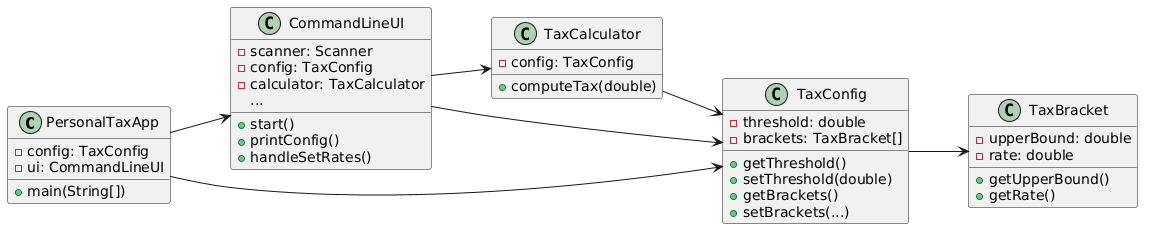
\includegraphics[width=\textwidth]{image/UML.png}
    \caption{主要类的 UML 类图}
    \label{fig:uml}
\end{figure}

各类关系说明：
\begin{itemize}
    \item \textbf{PersonalTaxApp}：主程序入口，负责初始化配置和启动命令行界面。
    \item \textbf{CommandLineUI}：命令行交互界面，负责菜单、输入输出、配置展示和用户操作。
    \item \textbf{TaxCalculator}：核心计算类，依赖 TaxConfig 进行分段累进税额计算。
    \item \textbf{TaxConfig}：保存起征点和税率档位，支持动态调整。
    \item \textbf{TaxBracket}：单一税率档次，包含上限和税率。
\end{itemize}

类之间通过组合和依赖关系协作，体现了高内聚、低耦合和分层设计思想。
\subsection{面向对象程序设计}

本项目严格遵循面向对象程序设计（OOP）思想，具体体现在以下几个方面：
\begin{itemize}
	\item \textbf{抽象与分层}：将个人所得税计算问题抽象为多个类，每个类只负责自身的职责。例如，\texttt{TaxCalculator} 只负责税额计算，\texttt{TaxConfig} 负责税率和起征点配置，\texttt{TaxBracket} 表示单一税率档次，\texttt{CommandLineUI} 负责用户交互。
	\item \textbf{封装与信息隐藏}：各类的属性均为私有（private），通过公有方法（getter/setter）访问和修改，防止外部直接操作内部数据，保证数据安全和一致性。
	\item \textbf{可扩展性与复用性}：税率表、起征点等均通过配置类实现，便于后续政策调整或功能扩展。各类之间低耦合高内聚，便于单独测试和复用。
	\item \textbf{异常处理}：通过抛出和捕获异常，保证系统健壮性，体现了面向对象对异常的统一管理。
	\item \textbf{主入口与分工}：\texttt{PersonalTaxApp} 作为主入口，负责启动配置和界面，体现了面向对象的分工协作思想。
\end{itemize}
整体设计不仅提升了代码的可维护性和可读性，也为后续功能扩展（如支持多种税制、图形界面等）提供了良好基础。

\subsection{类结构说明}
\begin{itemize}
	\item \textbf{TaxCalculator}：核心计算逻辑，实现分段累进税率的个税计算
	\item \textbf{TaxBracket}：税率等级定义，包含上限和税率
	\item \textbf{TaxConfig}：可配置的起征点和税率，支持动态调整
	\item \textbf{CommandLineUI}：命令行用户交互界面，负责菜单、输入输出和异常处理
	\item \textbf{PersonalTaxApp}：主程序入口
\end{itemize}
\subsection{主要流程}
\begin{enumerate}
	\item 启动程序，显示主菜单
	\item 用户选择功能：计算个税、设置起征点、设置税率、查看配置、退出
	\item 根据用户输入，调用相应方法，进行输入校验和异常处理
	\item 输出计算结果或配置信息
\end{enumerate}
\subsection{异常处理与健壮性}
所有用户输入均进行类型和范围校验，防止负数、非法字符等异常输入导致程序崩溃。对于无效输入，系统会给出友好提示并允许重新输入。

具体实现包括：
\begin{itemize}
	\item \textbf{输入校验：} 对工资收入、起征点、税率等输入进行类型（如必须为数字）、范围（如收入不能为负数、税率在合理区间）校验，防止非法数据进入计算流程。
	\item \textbf{单元测试覆盖：} 通过 JUnit 单元测试，覆盖了正常、边界和异常情况。例如：收入为0或低于起征点时税额为0，分段边界计算正确，负收入、负起征点、税率数组长度不符等均能正确抛出异常并提示。
	\item \textbf{健壮性验证：} 所有测试用例均通过，异常情况均被正确捕获和提示，保证了系统的健壮性。
\end{itemize}

\chapter{测试结果}

\section{命令行程序美观性与操作说明}
程序菜单采用分隔线和对齐输出，界面简洁美观，所有输入均有中文提示。错误输入时有醒目提示，用户体验良好。

\section{单元测试与异常处理}
本项目采用 JUnit 4 作为单元测试框架，测试类 \texttt{TaxCalculatorTest.java} 覆盖了正常、边界和异常情况。测试情况如下：
\begin{itemize}
	\item 收入为0或低于起征点，税额为0
	\item 收入处于各级分段边界，分段计算结果正确
	\item 设置负数起征点、税率数组长度不符等，均能抛出异常
	\item 负收入输入时，自动检测并抛出异常，防止非法数据进入计算流程
\end{itemize}

在给定的测试，张三某月工资薪金总收入为 4,300 元，减去免征基数 1,600 元，则应纳税所得额为 2,700 元。
于是我进行了如下几个测试：
\begin{table}[htbp]
    \centering
    \begin{tabular}{|c|c|c|c|}
    \hline
    测试用例 & 输入收入 & 期望税额 & 实际税额 \\
    \hline
    TC1 & 0 & 0 & 0 \\
    TC2 & 1600 & 0 & 0 \\
    TC3 & 4300 & 280 & 280 \\
    TC4 & 5000 & 385 & 385 \\
    TC5 & -100 & 异常 & 异常 \\
    \hline
    \end{tabular}
    \caption{单元测试结果}
    \label{tab:test-results}
\end{table}

所有测试用例均通过，异常情况均被正确捕获和提示，保证了系统的健壮性。

\section{运行截图}
见附录。

\chapter{自我评分参照}

本实验自我评分标准如下表所示，并对每一项在报告中的对应章节进行了标注：


\begin{table}[htbp]
	\centering
	\begin{tabular}{|p{5cm}|c|c|p{5.5cm}|}
	\hline
	评分项目 & 权重 & 报告对应章节 \\
	\hline 
	 1. 基本功能需求 & & 第4章“实验内容” \\
	 1.1 可运行的程序 & 30\% & 4.1“基本要求实现”、4.2“个人所得税计算方法” \\
	 2. 编程风格  &  & 第2章“实验环境” \\
	2.1 标识符命名 & 6\% & 2.3“编码规范-标识符命名” \\
	2.2 文档化注释 & 6\% & 2.4“编码规范-文档化注释” \\
	2.3 程序版面 & 3\% & 2.5“编码规范-程序版面” \\
	3. 结构化程序设计&  & 4.3“系统设计与实现” \\
	3.1 子程序功能划分 & 10\% & 4.3.3“类结构说明” \\
	3.2 子程序接口设计 & 5\% & 4.3.3“类结构说明”、4.3.4“主要流程” \\
	3.3 控制结构运用 & 5\% & 4.3.4“主要流程” \\
	4. 面向对象程序设计&   & 4.3“系统设计与实现” \\
	4.1 类的提炼与建模 & 5\% & 4.3.1“UML表示”、4.3.3“类结构说明” \\
	4.2 类的属性与行为设计 & 5\% & 4.3.3“类结构说明” \\
	4.3 访问控制设计 & 5\% & 4.3.2“面向对象程序设计” \\
	4.4 异常处理 & 5\% & 4.3.5“异常处理与健壮性”、5.2“单元测试与异常处理” \\
	5. 实验报告&   & 全文，重点第1、2、3、4、5章 \\
	5.1 实验报告内容 & 4\% & 全文 \\
	5.2 UML表示 & 3\% & 4.3.1“UML表示” \\
	5.3 文档与源程序组织 & 3\% & 第3章“项目文件组织” \\
	6. 其他&  & 5.2“单元测试与异常处理”、5.3“运行截图” \\
	6.1 测试用例及测试结果 & 5\% & 5.2“单元测试与异常处理”、5.3“运行截图” \\
	\hline
	\end{tabular}
	\caption{评分项目与对应报告章节}
	\label{tab:self-eval-map}
\end{table}


\chapter{实验总结}
本实验通过设计与实现一个命令行个人所得税计算器，达成了预定的教学目标：把现实问题抽象为若干类与模块，强化封装与信息隐藏思想，并掌握异常处理与输入校验的实现技巧。

在实现过程中，采用了 `TaxConfig`、`TaxBracket`、`TaxCalculator` 与 `CommandLineUI` 等模块化设计，清晰划分了配置、计算与交互职责。这种分层设计提高了代码的可维护性与可测试性，便于单元测试和后续扩展。核心计算逻辑使用分段超额累进税率实现，并提供了对起征点和税率的动态调整功能。

为保证程序健壮性，我们对用户输入进行了严格校验，添加了异常捕获与友好提示，同时编写了 JUnit 测试用例覆盖正常、边界与异常情况（如负收入、起征点异常、税率配置错误等）。在示例测试中，月收入 4300 元、起征点 1600 元时的计算结果与预期一致，验证了实现的正确性。

通过本次实验，收获包括：
\begin{itemize}
	\item 理解并实践了面向对象分析与设计在小型工程中的应用；
	\item 熟练掌握了 Java 中异常处理、输入校验与单元测试的常用模式；
	\item 学会将配置与业务逻辑分离，以提升系统可扩展性；
	\item 加强了编写文档化注释与保持代码风格一致的重要性。
\end{itemize}

后续可改进与扩展的方向包括：支持按年或按多项收入汇总的税制、添加持久化配置文件或 GUI 界面、以及引入更完善的国际化与本地化支持。这些改进将进一步考验模块化设计的灵活性并提升用户体验。

综上所述，本实验既巩固了编译原理关联的程序结构与数据流观念，也显著提升了面向对象编程与工程化实践能力。
